\documentclass[A4paper, 11pt]{article}

\usepackage[UTF8]{ctex}
\usepackage{amsfonts}
\usepackage{amsmath} 
\usepackage{amssymb}
\usepackage{array}
\usepackage{booktabs}
\usepackage{bm}
\usepackage{cite}
\usepackage{colortbl}
\usepackage{enumerate}
\usepackage{extarrows}
\usepackage{float}
\usepackage{geometry}
\usepackage{graphics}
\usepackage{graphicx}
\usepackage{ifthen}
\usepackage{listings}
\usepackage{longtable}
\usepackage{multicol}
\usepackage{pgf}
\usepackage{pgfplots}
\usepackage{pifont}
\usepackage{pstricks}
\usepackage{pst-node}
\usepackage{pst-tree}
\usepackage{pythonhighlight}
\usepackage{setspace}
\usepackage{tabularx}
\usepackage{tikz}
\usepackage{tocloft}
\usepackage{wrapfig}

\geometry{left=2cm, right=2cm, top=2cm, bottom=2cm}

\definecolor{emph}{RGB}{0,100,141}

\newcommand{\tabincell}[2]{\begin{tabular}{@{}#1@{}}#2\end{tabular}}
\newcommand*{\circled}[1]{\lower.7ex\hbox{\tikz\draw (0pt, 0pt) circle (.5em) node {\makebox[1em][c]{\small #1}};}}
\newcommand{\sfrac}[2]{\mbox{\small$\dfrac{#1}{#2}$}}
\renewcommand{\geq}{\geqslant}
\renewcommand{\leq}{\leqslant}
\renewcommand{\vec}{\overrightarrow}
\renewcommand{\d}{\,\mathrm{d}}
\newcommand{\lto}{\longrightarrow}
\newcommand{\ex}{\exists\,}
\newcommand{\R}{\mathbb{R}}
\newcommand{\<}{\,\langle\,}
\renewcommand{\>}{\,\rangle}
\newcommand{\normuv}[1]{\big|{#1}(u,v)\big|^2}
\newcommand{\infint}{\int_{-\infty}^{+\infty}}
\newcommand{\hollowstar}{\text{\ding{73}}}
\newcommand{\fullstar}{\text{\ding{72}}}

\newcommand{\Pro}[1]{\textbf{\large{Problem #1}} \vspace*{1ex}}
\newcommand{\Sol}{\textbf{\textit{Sol.}}}
\newcommand{\Ckp}{\textbf{\textit{Checkpoints}}}
\newcommand{\Pt}[1]{\textcolor{emph}{(#1 \ifthenelse{\equal{#1}{1}}{point}{points})}}

% Scalars
\renewcommand{\a}{\alpha}
% Matrices
\newcommand{\A}{\bm{A}}
\newcommand{\B}{\bm{B}}
\newcommand{\C}{\bm{C}}
\newcommand{\E}{\bm{E}}
% Vectors
\renewcommand{\b}{\bm{b}}
\newcommand{\x}{\bm{x}}
\newcommand{\y}{\bm{y}}
\newcommand{\z}{\bm{z}}
\renewcommand{\u}{\bm{u}}
\renewcommand{\v}{\bm{v}}
\newcommand{\w}{\bm{w}}
\newcommand{\0}{\mathbf{0}}
\newcommand{\1}{\mathbf{1}}
% Spaces
\newcommand{\V}{\mathcal{V}}
\newcommand{\X}{\mathcal{X}}
\newcommand{\Y}{\mathcal{Y}}
\newcommand{\F}{\mathcal{F}}
\newcommand{\N}{\mathcal{N}}
\renewcommand{\S}{\mathcal{S}}
% Names
\renewcommand{\sp}{\text{span}}
\newcommand{\rank}{\text{rank}}
\newcommand{\range}{\mathcal{R}}
\newcommand{\tr}{\text{tr}}

\newcommand{\typeset}{
    \setlength{\parindent}{0pt}
    \setlength{\parskip}{1ex}
    \setlength{\abovedisplayskip}{1ex}
    \setlength{\belowdisplayskip}{1ex}
}

\newcommand{\headbox}{
    \renewcommand{\arraystretch}{1.33}
    \begin{tabular}{|l|l|}
    \hline
    Name       & \hspace*{9em} \\
    \hline
    Student ID & \hspace*{9em} \\
    \hline
    \end{tabular} \hspace{131pt}
    \begin{tabular}{r}
        \textsc{CS\,270:\;Digital\;Image\;Processing} \\
        \textbf{\Large{Quiz 1}} \\
    \end{tabular}
    
    \vspace*{6ex}
    \renewcommand{\arraystretch}{1}
}

\begin{document}

\begin{spacing}{1.3}

\typeset

\textsc{\large{School\;of\;Information\;Science\;and\;Technology\\[2pt] ShanghaiTech\;University}}

\vspace*{5ex}

\textsc{\large{CS\,270:\;Digital\;Image\;Processing (Spring\;2024)}}

\vspace*{2.5ex} \textbf{\huge{Assignment 1}}

\vspace*{1.5ex} \textbf{\large{Due: 23:59, April 7, 2024}}

\vspace*{5ex}

\textbf{\large{Notes}}

\begin{itemize} \setlength{\parskip}{0.5ex} \vspace*{-1ex} 
    \item This assignment has \textbf{100 points} in total.
    \item Please prepare all your solutions in English.
    \item Please prepare your report with digital typesetting software (LaTeX, Microsoft Word, etc.). Handwritten reports, including digital handwriting on iPad etc., will not be accepted.
    \item Please submit your assignment to \textbf{Blackboard} as a \textbf{zip} file with its name formatted as\\ \texttt{DIP2024\_HW1\_ID\_ChineseName.zip}. The zip file should contain 3 things:
    \begin{enumerate}
        \item Your report named as \texttt{HW1\_Report\_ID\_Name.pdf};
        \item A folder named as \texttt{code} that stores your codes;
        \item A folder named as \texttt{images} that stores the original images in your report.
    \end{enumerate}
    For each problem, you should provide a separate code file that corresponds to it, with its name like \texttt{p3.m} (for Problem 3) or \texttt{p6a.m} (for Problem 6 (a)). Please make sure all paths in your codes are relative paths, so that we can run your codes and get your results without any modification.
\end{itemize}

\vspace*{2ex}
\textbf{\large{Policy on Plagiarism}}
\vspace*{1.5ex}

This is an individual homework. You can discuss the ideas and algorithms, but:
\begin{itemize} \setlength{\parskip}{0.5ex} \vspace*{-1.5ex}
    \item You cannot read, modify, and submit the codes of other students, nor allow other students to read, modify, and submit your codes.
    \item You cannot directly use generative AI tools to produce codes for submission. While you may consult generative AI for understanding the ideas and algorithms, the code you submit must be the result of your own individual understanding and efforts.
\end{itemize} \vspace*{-1.5ex}
We will utilize automated tools to check for plagiarism, and any violations will result in a zero score for this assignment and $20\%$ discount on total course grade.

\newpage

\begin{center}
    \textsc{I. Coding Part}
\end{center}

Please complete all the coding assignments using MATLAB. Make sure your results in the report are the same as the results of your codes. For general operations, the following functions may be useful:\\
\texttt{load}, \texttt{imread}, \texttt{double}, \texttt{im2double}, \texttt{uint8}, \texttt{imshow}, \texttt{zeros}, \texttt{size}, \texttt{montage}, \texttt{subplot}, \texttt{bar}.

\textcolor{red}{You must implement the core code in each question WITHOUT using relevant build-in functions, e.g,}\\
\textcolor{red}{
\texttt{fspecial}, \texttt{imfilter}, \texttt{filter2}, \texttt{conv2}, \texttt{imsharpen}, \texttt{ordfilt2}, \texttt{hist}, \texttt{imadjust}, \texttt{histeq}, \texttt{adapthisteq},~etc.
}

\vspace*{-3.75ex}
You can type \texttt{\textbf{help} FunctionName} in Command Window of MATLAB for detailed help text for the functionality specified by \texttt{FunctionName}.

\vspace*{6ex}

\Pro{1: Histogram Equalization}


\begin{enumerate}[\bfseries(a)] \setlength{\parskip}{0.5ex} \vspace*{-2ex}
    \item Compute the histogram of \texttt{grain.tif} and show the histogram image in your report. (Built-in functions \texttt{hist} and \texttt{histogram} are not allowed). \Pt{5}
    \item Implement histogram equalization on \texttt{grain.tif}. Show the histogram equalized image and the histogram of equalized image in your report. (Built-in function \texttt{histeq} is not allowed). \Pt{10}
    \item Implement contrast limited adaptive histogram equalization (CLAHE) on \texttt{grain.tif}, where you traverse every pixel with a $40 \times 40$ patch and process histogram equalization within each patch and update the center patch of $3 \times 3$. Each time you move the patch with a step of 1 pixel. The clip limit for CLAHE is 0.02, which means that after the normalization of the histogram, amplification above 0.02 should be clipped and evenly distributed to other parts of the histogram. Show the CLAHE processed images and corresponding histogram in your report. (Built-in function  \texttt{adapthisteq} is not allowed)  \Pt{20}
\end{enumerate}

\begin{figure}[h]
        \centering
        \begin{minipage}[t]{0.4\textwidth}
        \centering
        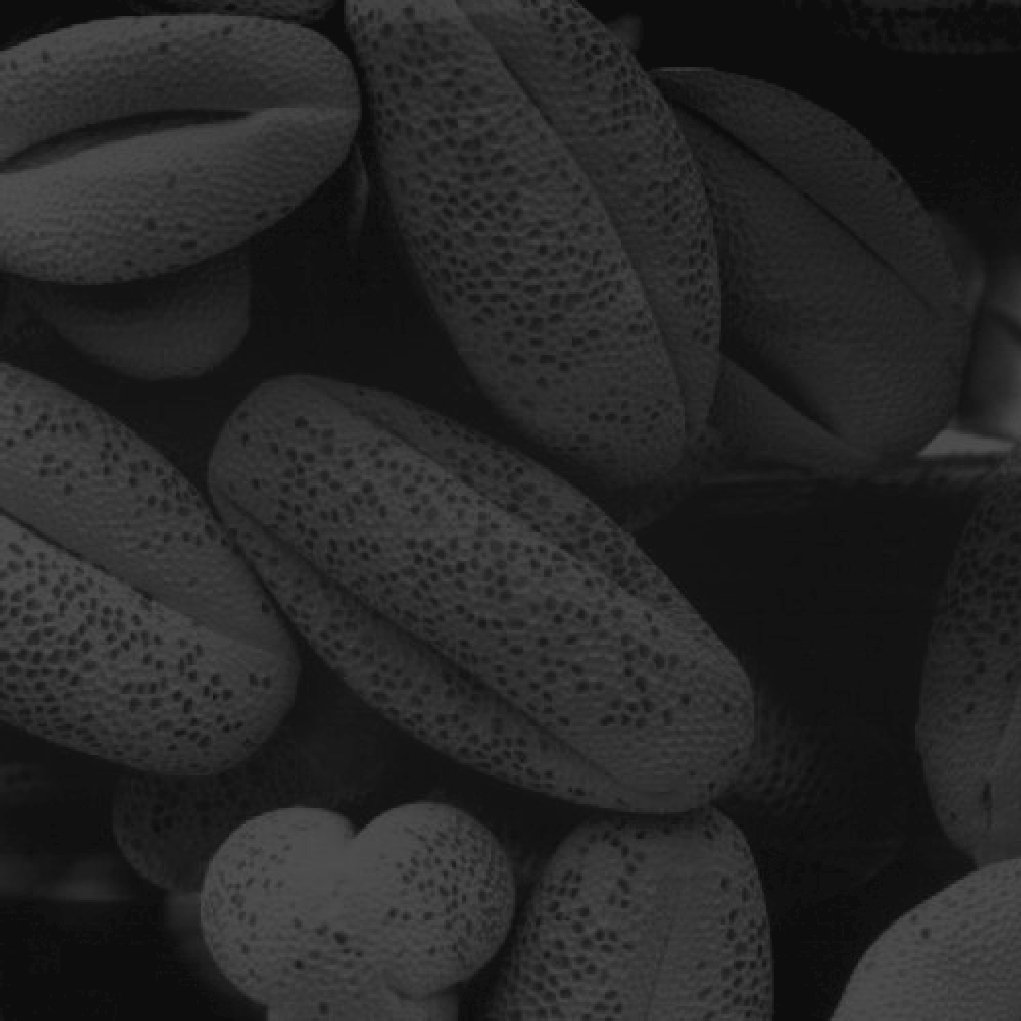
\includegraphics[height=5cm]{../origin_images/grain.jpg}
        \end{minipage}
        \begin{minipage}[t]{0.4\textwidth}
        \centering
        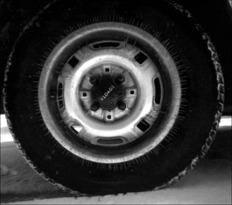
\includegraphics[height=5cm]{../origin_images/tire.jpg}
        
        \end{minipage}
    \end{figure}
    

\newpage

\Pro{2: Image Sharpening}

(a) Apply the $3\times 3$ Laplacian kernels ($x$-direction and $y$-direction) on \texttt{moon.jpg} to obtain the details of the image. Since the Laplacian kernels are separable, please separate them into combinations of 1-D kernels and then apply them to the image sequentially. Show the separated Laplacian kernels and the corresponding processed images. (Implement your own \textbf{convolution} operator.) \Pt{15}

(b) Apply the $3\times 3$ Laplacian kernels (not separated) to sharpen the image by 2-D convolution. Show the results in your report. \Pt{10}

(c) Use unsharpen mask to sharpen the image. Show the results in your report. \Pt{10}

The pixel intensity of the result images should be normalized to \texttt{uint8} values within $[0, 255]$.

\begin{center}
    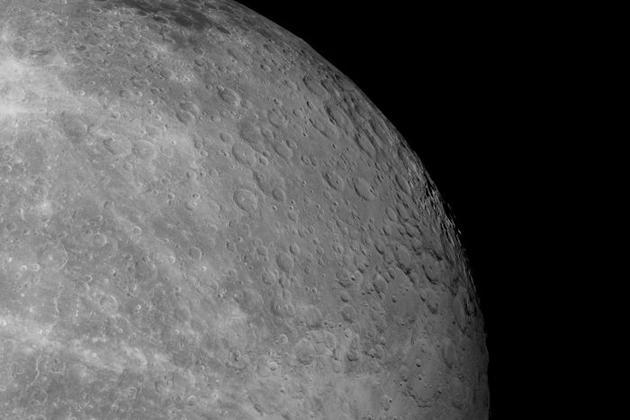
\includegraphics[width=5.5cm]{../origin_images/moon.jpg}
\end{center}

\newpage


\Pro{3: Nonlinear Filter}

Apply the median filter and Gaussian filter to the image \texttt{lena\_noisy.tif}. In your report, Please show the images processed by the median filter and Gaussian filter respectively, and analyze the cause of the results. (Filtering operations cannot be implemented by calling functions, Hint: Choose the best kernel size you think, $\sigma = 1$) \Pt{30}

\begin{center}
    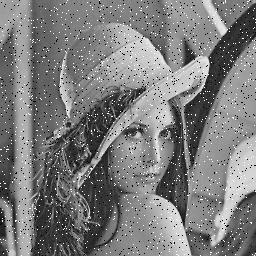
\includegraphics[height=5.5cm]{../origin_images/lena.jpg}
\end{center}

\newpage




\end{spacing}

\end{document}